
La loi de Wien décrit la relation liant la longueur d'onde  $\lambda_{max}$, correspondant au pic d'émission lumineuse du corps noir, et la température $T$ (exprimée en kelvin). Voici la courbe pour quelques températures.

\begin{center}
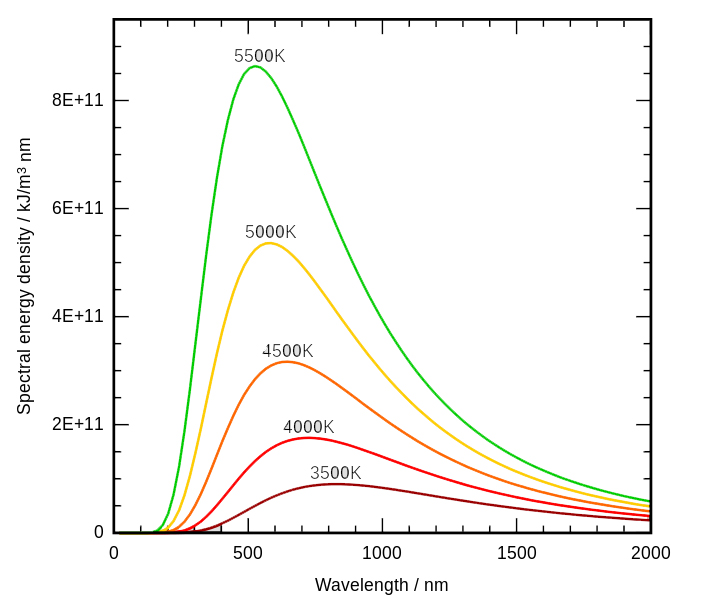
\includegraphics[scale=0.4]{FEA-52.jpg} 
\end{center}

\begin{enumerate}
\item Lire la densité spectrale d'énergie pour une longueur d'onde de $500 nm$ et une température de $4000K$.
\item Lire la Température lorsque la densité spectrale est de $2.10^{11} KJ/m^3 nm$ et la longueur d'onde de $1200 nm$.
\item Lire la longueur d'onde pour une température de $5000K$ et une densité spectrale de $4.10^{11} KJ/m^3 nm$.
\end{enumerate}

\PESP{https://fr.wikipedia.org/wiki/Loi\_du\_d\%C3\%A9placement\_de\_Wien}